\documentclass[11pt,a4paper]{ctexart}

\usepackage[margin=2.6cm]{geometry}
\usepackage{amsmath,amssymb,amsthm}
\usepackage{graphicx}
\usepackage{booktabs}
\usepackage{hyperref}
\usepackage{xcolor}
\usepackage{listings}
\usepackage{caption}

\graphicspath{{figures/}}
\hypersetup{colorlinks=true, linkcolor=blue!50!black, urlcolor=blue!60!black}
\lstset{
  basicstyle=\ttfamily\small,
  breaklines=true,
  frame=single,
  columns=fullflexible,
  backgroundcolor=\color{gray!7}
}

\title{第 1 章 \quad Introduction / 导论}
\author{基于 \textit{A Course in Time Series Analysis} 的中文讲义与 Python 实践}
\date{}

\begin{document}
\maketitle

\section*{本章学习目标}

本章的作用是建立时间序列分析的入口视角。原文从最简单的独立随机变量出发，说明时间序列与经典统计的核心差别：观测值按照时间排序，并且相邻或相隔若干期的观测之间常常存在依赖结构。正是这种依赖结构，使预测、滤波、趋势识别和周期识别成为可能。

完成本章后，应能够：
\begin{itemize}
  \item 说明什么是等间隔观测的时间序列；
  \item 区分无相关随机序列和具有时间结构的真实序列；
  \item 理解 SOI、Nasdaq、太阳黑子、气温等数据在时间序列课程中的典型用途；
  \item 将原文中的 R 入门绘图思路改写为 Python 实践；
  \item 理解线性滤波的基本表达式以及它在后续章节中的作用。
\end{itemize}

\section{时间序列的基本概念}

时间序列是一组按时间顺序记录的观测值，记作
\[
  x_t,\quad t \in \mathbb{Z}.
\]
观测方式可以有多种：在一个连续区间上观测、在区间中随机抽样观测，或者在固定的等间隔时间点观测。本课程主要讨论第三种情形，即观测点之间间隔相同。为了便于数学表达，通常将时间下标写成整数集合
\[
  \mathbb{Z}=\{\ldots,-1,0,1,2,\ldots\}.
\]

最简单的时间序列是独立同分布随机变量序列。如果每个观测之间相互独立且均值为 0，那么从图形上通常看不到稳定的趋势、周期或可利用的依赖结构。此时，对下一期观测的最佳朴素预测往往只是均值 0。

\begin{figure}[htbp]
  \centering
  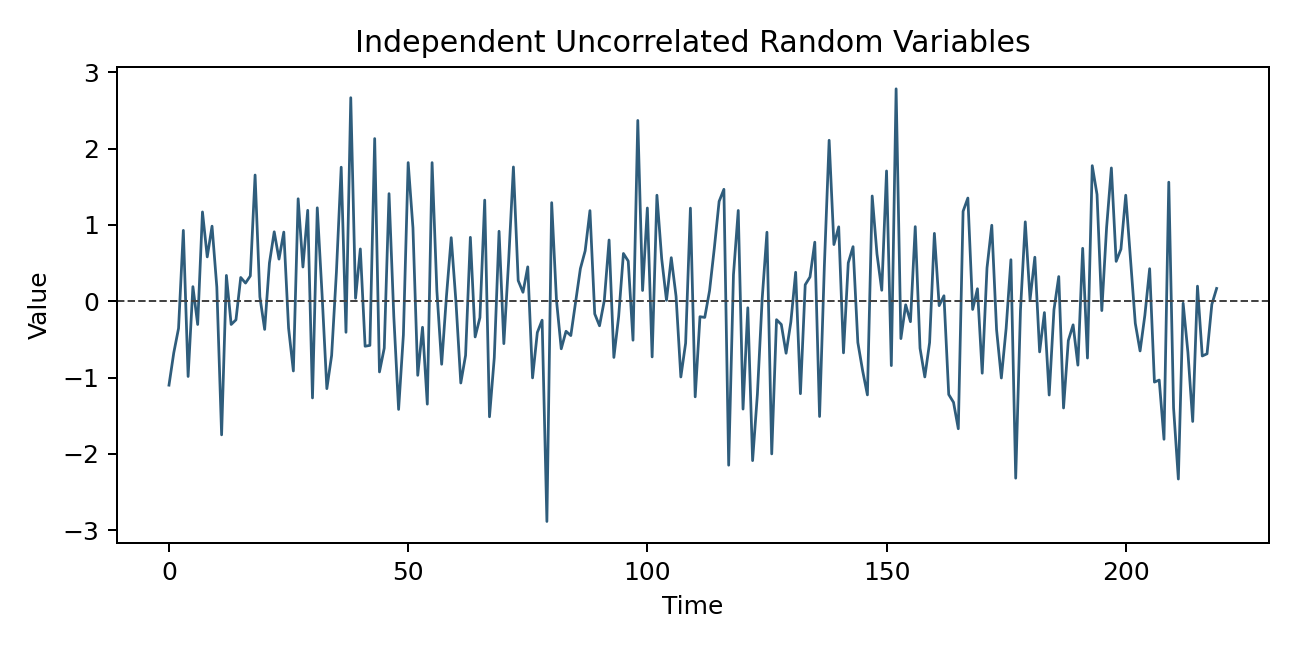
\includegraphics[width=0.86\textwidth]{ch01_fig01_white_noise.png}
  \caption{独立无相关随机变量序列。该图对应原文 Figure 1.1 的教学意图：序列围绕 0 上下波动，但没有明显趋势或周期。}
\end{figure}

时间序列分析真正关心的是观测之间的依赖。若当前值与过去值相关，过去信息就可能帮助我们预测未来；若序列中存在周期结构，我们可以识别周期；若均值随时间缓慢变化，我们需要估计趋势。

\section{典型时间序列数据}

原文用四类数据说明时间序列问题的多样性。

\subsection{南方涛动指数}

南方涛动指数（Southern Oscillation Index, SOI）描述塔希提和达尔文之间海平面气压差的波动，是衡量厄尔尼诺现象强度的重要指标之一。原文使用 1876 年 1 月到 2014 年 7 月的月度 SOI 数据，并强调一个主要目标：寻找数据中的模式，特别是周期性。

在没有直接附带原始 SOI 数据文件的情况下，本章 Python 脚本生成一个具有周期成分和持续性噪声的模拟 SOI 序列，用于复现“月度气候指标具有波动结构”的教学场景。

\begin{figure}[htbp]
  \centering
  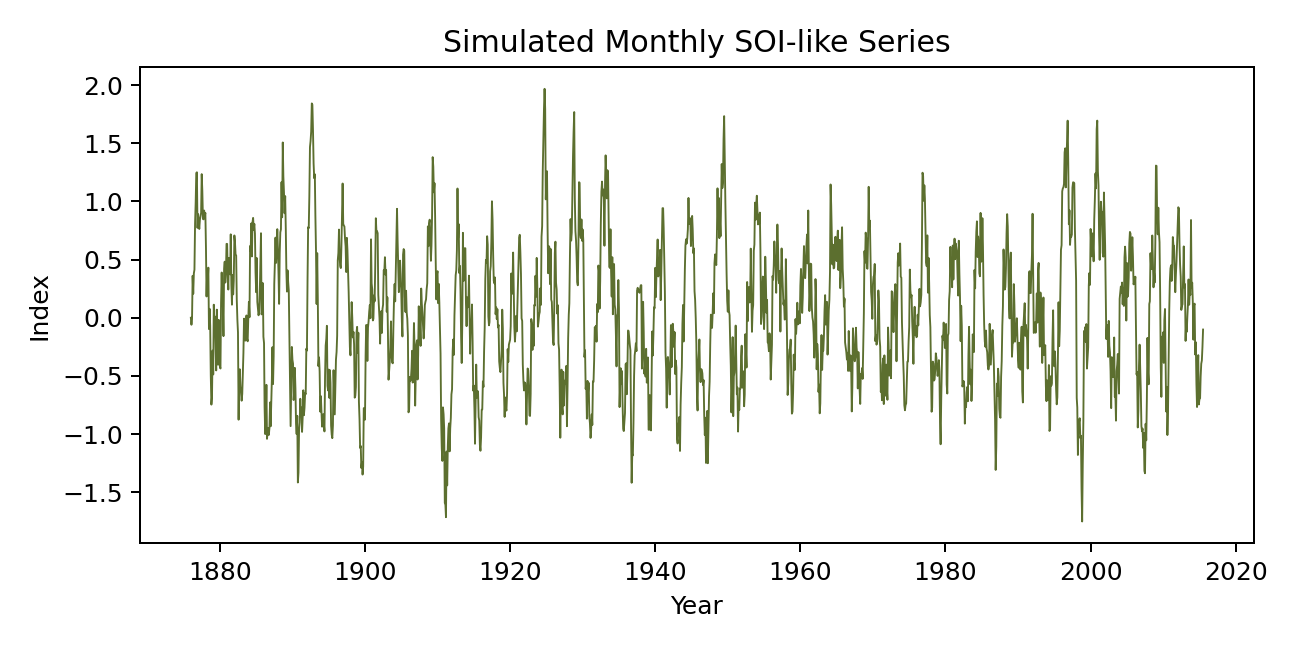
\includegraphics[width=0.86\textwidth]{ch01_fig02_simulated_soi.png}
  \caption{模拟的月度 SOI 型序列。图中可见慢周期波动和持续性噪声，这类结构适合引出周期检测和相关噪声问题。}
\end{figure}

\subsection{Nasdaq 金融数据}

原文展示了 1985 年 10 月 1 日至 2014 年 8 月 8 日的 Nasdaq 日收盘价。金融时间序列的直接动机常常是预测收益、风险或波动率。对于价格序列本身，常见现象包括长期增长、非平稳性和波动聚集；后续章节会逐步讨论差分、ARMA、ARCH/GARCH 等工具。

\subsection{太阳黑子数据}

太阳黑子数量是经典时间序列案例。太阳活动具有明显的周期性，因此适合用来引出周期识别、谱分析和长期预测。下面的 Python 图使用 \texttt{statsmodels} 内置太阳黑子数据。

\begin{figure}[htbp]
  \centering
  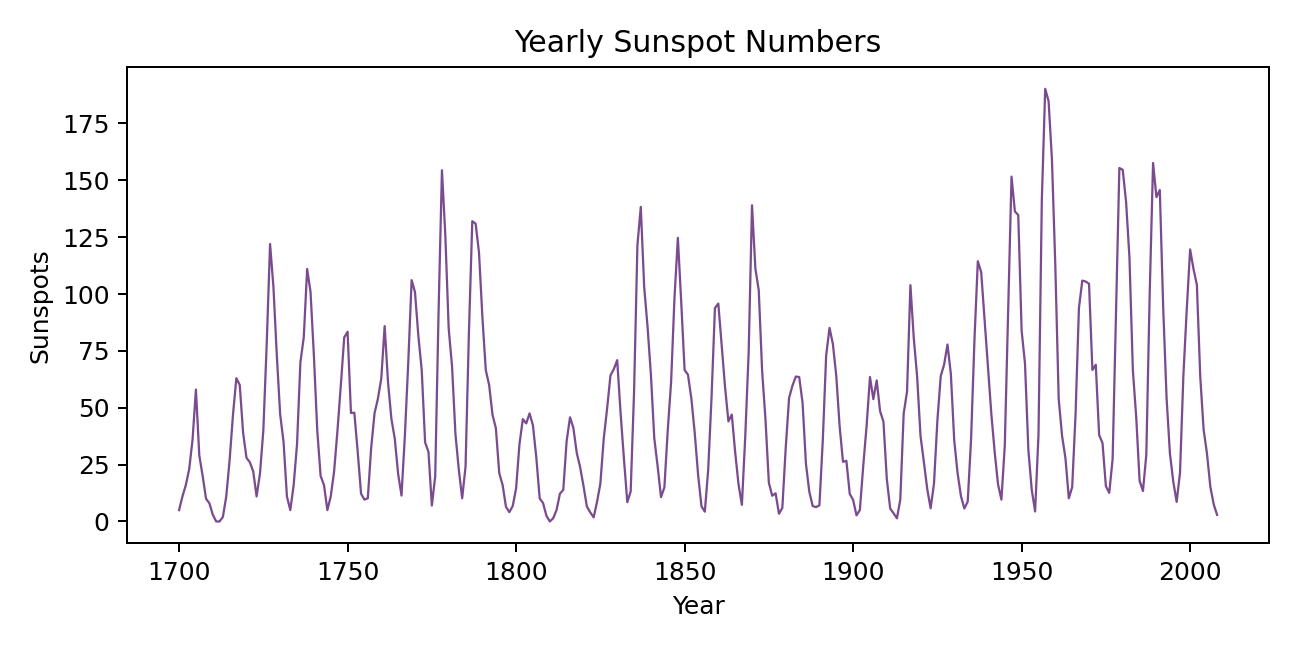
\includegraphics[width=0.86\textwidth]{ch01_fig03_sunspots.png}
  \caption{年度太阳黑子数量。可观察到明显的周期波动，是后续研究周期和谱密度的典型案例。}
\end{figure}

\subsection{年度与月度气温数据}

气温异常序列常用于研究长期均值变化。原文指出，若目标是检测全球变暖，就不能只画一条趋势线后直接下结论，还需要时间序列统计推断来判断趋势估计是否显著。原因在于，时间序列观测通常不是独立样本，相关性会改变估计量的标准误和显著性判断。

\section{从 R 代码到 Python 实践}

原文提醒读者熟悉 R，并给出了 \texttt{ts()} 和 \texttt{plot.ts()} 的基本用法。在 Python 中，类似工作通常由 \texttt{pandas} 的时间索引、\texttt{matplotlib} 绘图和 \texttt{statsmodels} 建模共同完成。

\begin{lstlisting}[language=Python, caption={Python 中构造月度时间序列的基本模式}]
import pandas as pd

dates = pd.date_range("1876-01-01", periods=120, freq="MS")
series = pd.Series(range(120), index=dates)
series.plot()
\end{lstlisting}

本章的完整实践脚本位于：
\[
  \texttt{scripts/ch01\_generate\_figures.py}.
\]
运行后会在 \texttt{figures/} 目录生成本章所有图像。

\section{时间序列滤波}

为了突出某些特征或去除不需要的特征，我们经常对原始时间序列做变换。原文特别强调线性变换。设原始序列为 \(\{X_t\}\)，变换后的序列为 \(\{Y_t\}\)，则线性滤波可以写作
\[
  Y_t = \sum_{j=-\infty}^{\infty} h_j X_{t-j},
\]
其中 \(\{h_j\}\) 是一组权重。

本课程后续主要使用两类线性变换：
\begin{itemize}
  \item 用于估计随时间变化的均值函数，例如移动平均平滑；
  \item 用于理解观测序列中的随机部分，例如频域变换和滤波。
\end{itemize}

\begin{figure}[htbp]
  \centering
  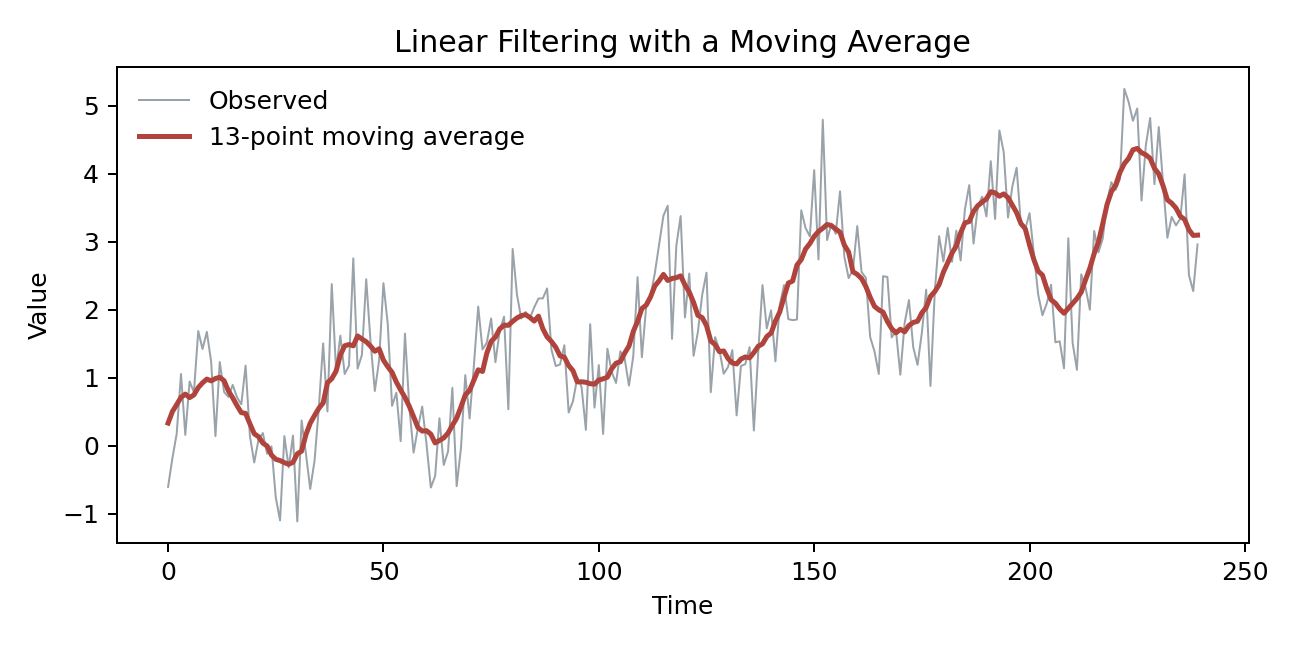
\includegraphics[width=0.86\textwidth]{ch01_fig04_filtering.png}
  \caption{移动平均滤波示例。灰色曲线是带噪声观测，红色曲线是 13 点移动平均，展示了线性滤波如何突出低频趋势。}
\end{figure}

\section{术语}

\begin{description}
  \item[iid] independent and identically distributed，独立同分布。它是最简单的时间序列模型，但通常不是实际时间序列分析的终点。
  \item[预测] 利用过去和当前信息推断未来观测。
  \item[趋势] 序列均值随时间发生的系统性变化。
  \item[周期] 序列中以某种频率重复出现的结构。
  \item[滤波] 通过加权组合过去、当前或未来观测来变换序列。
\end{description}

\section{Python 工程实践说明}

在本章目录下运行：
\begin{lstlisting}[language=bash]
python scripts/ch01_generate_figures.py
\end{lstlisting}

脚本生成四张图：
\begin{itemize}
  \item \texttt{ch01\_fig01\_white\_noise.png}：独立无相关随机序列；
  \item \texttt{ch01\_fig02\_simulated\_soi.png}：模拟 SOI 型月度序列；
  \item \texttt{ch01\_fig03\_sunspots.png}：太阳黑子年度序列；
  \item \texttt{ch01\_fig04\_filtering.png}：移动平均滤波。
\end{itemize}

\section*{本章小结}

第 1 章的重点不是推导复杂模型，而是建立问题意识：时间序列数据的顺序和依赖结构很重要。独立随机变量序列几乎没有可预测结构，而气候、金融、太阳活动和温度序列往往具有趋势、周期、波动聚集或相关噪声。后续章节会围绕这些结构展开：先研究趋势，再研究平稳性、线性模型、预测、估计、谱分析和非线性模型。

\end{document}

